\documentclass[11pt,oneside,a4paper]{memoir}
\usepackage{fontspec}
\usepackage{xltabular}
\usepackage{graphicx}
\usepackage[unicode=true,xetex,colorlinks=true,linkcolor=blue,urlcolor=blue,bookmarksnumbered=true,bookmarksdepth=3]{hyperref}
\usepackage{bidi} % Must be last


%%%%%%%%%%%%%%%%%%%%%%%%%%%%%%%%%%%%%%%%%%%%%%%%%%%%%%%
%%%%%%%%%%%%%%%%%%%% Configuration %%%%%%%%%%%%%%%%%%%%
%%%%%%%%%%%%%%%%%%%%%%%%%%%%%%%%%%%%%%%%%%%%%%%%%%%%%%%

%%% Fonts %%%
\setmainfont[Ligatures=TeX]{Linux Libertine O}
\newfontfamily{\ezr}[Script=Hebrew]{EzraSIL}

\newfontfamily{\mainnolig}{Linux Libertine O}
\newcommand{\q}{{\mainnolig '}}


%%% Page layout %%%
\settypeblocksize{247mm}{160mm}{*}
\setlrmargins{*}{*}{1}
\setulmargins{*}{*}{1}
\checkandfixthelayout

%%% Hyperref (Information in PDF) %%%
\hypersetup{
unicode=true,
pdfauthor={Claus Tøndering},
pdftitle={Bible Online Learner: Localization Guide}
}

%%% Section numbering %%%
\setsecnumdepth{section}

%%% Lists %%%
\tightlists

%%% Chapter style %%%

% My own version of the ell chapter style:
\makechapterstyle{claus}{%
  \chapterstyle{default}
  \renewcommand*{\chapnumfont}{\normalfont\HUGE\sffamily}
  \renewcommand*{\chaptitlefont}{\normalfont\huge\sffamily}
  \settowidth{\chapindent}{\chapnumfont 111}
  \renewcommand*{\chapterheadstart}{\begingroup
    \vspace*{\beforechapskip}%
    \begin{adjustwidth}{}{-\chapindent}%
    \hrulefill
    \smash{\rule{0.4pt}{15mm}}
    \end{adjustwidth}\endgroup}
  \renewcommand*{\printchaptername}{}
  \renewcommand*{\chapternamenum}{}
  \renewcommand*{\printchapternum}{%
    \begin{adjustwidth}{}{-\chapindent}
    \hfill
    \raisebox{10mm}[0pt][0pt]{\chapnumfont\ifanappendix Appendix\else Chapter\fi\ \thechapter}%
                              \hspace*{1em}
    \end{adjustwidth}\vspace*{-3.0\onelineskip}}
  \renewcommand*{\printchaptertitle}[1]{%
    \vskip\onelineskip
    \raggedleft {\chaptitlefont ##1}\par\nobreak}}

% Default style should still use this font:
\renewcommand*{\chaptitlefont}{\normalfont\huge\sffamily}


\newenvironment{my-longtabx}[2]{
  \xltabular{\textwidth}{@{}#1@{}}
  \toprule
  #2\\
  \midrule
  \endfirsthead

  \toprule
  #2\\
  \midrule
  \endhead
  
  \emph{\rmfamily\normalsize(Continued...)} & \\
  \endfoot

  \bottomrule
  \endlastfoot
}{%
\endxltabular
}


\newcommand{\headii}[2]{\textbf{#1} & \textbf{#2}}
\newcommand{\headiii}[3]{\textbf{#1} & \textbf{#2} & \textbf{#3}}


%%% Allow extra space between words %%%
\sloppy


%%% Font matter %%%
\title{Bible Online Learner:\\Localization Guide}
\author{Claus Tøndering\\Ezer IT Consulting}
\date{13 December 2016}

%\makeindex


\begin{document}
\begin{titlingpage*}
\maketitle

\begin{center}
Copyright © 2016 by Claus Tøndering, claus@ezer.dk

\vspace{5mm}

The document is made available under a Creative Commons Attribution 4.0 International License

(see \url{http://creativecommons.org/licenses/by/4.0/})
\end{center}
\end{titlingpage*}


\clearpage
\tableofcontents
\chapterstyle{claus} % TOC should be in default style. "claus" style starts here.

%%%%%%%%%%%%%%%%%%%%%%%%%%%%%%%%%%%%%%%%%%%%%%%%%%%%%%
%%%%%%%%%%%%%%%%%%%% Introduction %%%%%%%%%%%%%%%%%%%%
\chapter{Introduction}

This document tells you how to create a translation of Bible Online Learner (Bible OL).

You are expected to be familiar with the way Bible OL is used, both by teachers and by students.

Before you start, you must have an account on the Bible OL website, and an administrator must grant
you ``translator'' privileges. Please be aware that as a translator you can modify all the available
translations, so be careful.

The system distinguishes between three types of translations:

\begin{enumerate}
\item The user interface, plus the grammatical terms for Hebrew and Greek.
\item The Hebrew and Aramaic lexicons.
\item The Greek lexicon.
\end{enumerate}

These three translations can be provided independently of one another.


\section{Creating a Translation for a New Language}

Bible OL already has translations for a number of languages, but if you want to add a new language,
you must follow these steps:

\begin{enumerate}
\item Contact me at claus@ezer.dk and request that a new language be enabled.
\item Provide the required translation.
\item Inform me when the translation is ready, and I will activate it.
\end{enumerate}


\section{Modifying a Translation for an Existing Language}

An existing language translation can be modified on the live system. The changes takes effect
immediately.


\section{Ongoing Work}

Please be aware that Bible OL is a dynamic program whose features change frequently. As new features
are added to the system, I will contact you and ask you to translate text for the new features.



%%%%%%%%%%%%%%%%%%%%%%%%%%%%%%%%%%%%%%%%%%%%%%%%%%%%%%%%%%%%%%%%%%%%%%%%
%%%%%%%%%%%%%%%%%%%% Translating the User Interface %%%%%%%%%%%%%%%%%%%%
\chapter{Translating the User Interface}

The term ``user interface'' here refers to the parts of the system that are not directly linked to a
Greek or Hebrew database.

To provide a translation, you must log in using an account that has ``translator'' privileges. Then,
from the ``Administration'' menu select ``Translate interface.''

You will then see a web page that looks something like this:

\begin{center}
  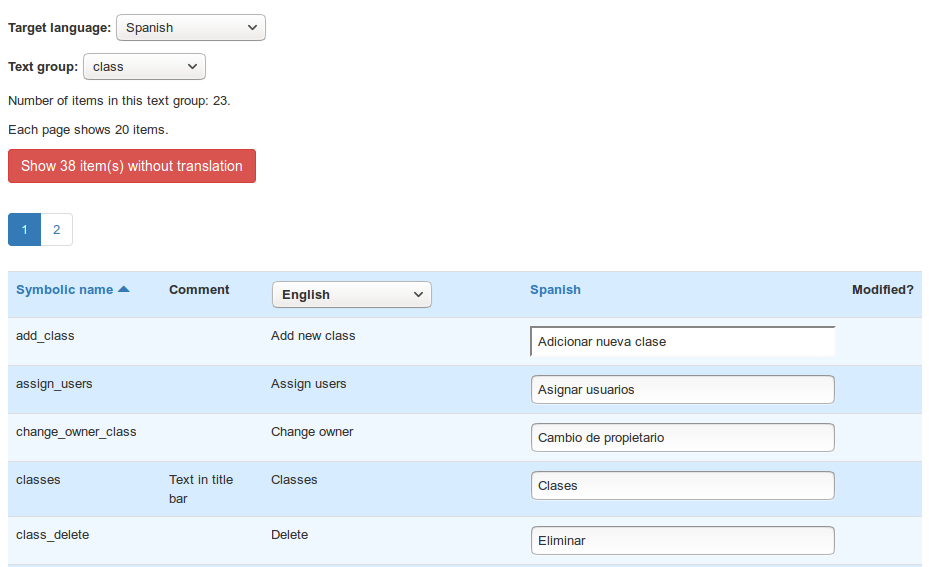
\includegraphics[width=0.9\linewidth]{interface.png}
\end{center}

From the drop-down menu labelled ``Target language'' select the language you are translating into.

For convenience, related texts are grouped in so-called ``text groups.'' You must provide a
translation for all text in all text groups. From the drop-down menu ``Text group,'' select the text
group you want to work with.

If there is text that you have not yet translated, clicking the red ``Show \ldots{} items without
translation'' will bring up a list of untranslated items.

The buttons labelled ``1'' and ``2'' in the above illustration allows you to switch between different
pages. If you have worked on one page, be sure to save it before you move to another page.

The area below the page buttons is divided into five columns:


\newcommand*{\labeli}[1]{\normalfont\bfseries #1}

\begin{flexlabelled}{labeli}{3cm}{*}{0cm}{4cm}{*}
\item[Symbolic name:\hfill] This is used internally by the system.
\item[Comment:] This column may provide some context for the translation.
\item[English (or some other language):] This is a drop down menu where you can select an existing
  language to use as the basis for your translation. It is highly recommended that you use English
  for this purpose; otherwise you will be working with something that is already a translation
  from English, and the result may not be the best.
\item[\emph{Target language:}\hfill]  Here you provide your translation.
\item[Modified?] If you have modified an entry, a ``Revert'' button will appear in the ``Modified?''
  column. If you click this button before you save your changes to the server, you will undo any
  changes you have made to that entry.
\end{flexlabelled}

You can click on the headings of the ``Symbolic name'' column or the target language column to change
the order of the items in the table. The fist time you click the heading, the items in that column
will be sorted in alphabetical order; the second time you click the heading, the items will be sorted
in reverse alphabetical order.

At the bottom of the screen, you will find two buttons, one labelled ``Submit changes'' and one
labelled ``Revert all.'' Clicking ``Submit changes'' will send your updated translations to the server;
clicking ``Revert all'' will undo all the changes you have made but not yet submitted.


\section{Special Characters}

\subsection{Punctuation Marks}

If the English string contains punctuation marks -- in particular if it ends with a colon -- you should
include similar punctuation in your own language if it makes sense. Be particularly conscious about
quotation mark styles, which can very greatly from language to language. For example:

\begin{itemize}
\item[] English: ``abc'' or `abc'
\item[] German: »abc« or ,,abc``
\item[] French: « abc »
\end{itemize}


\subsection{HTML Code}

In a few places the translated string may contain HTML commands. For example:

\begin{verbatim}
        Select number of questions<br>using preset passages
\end{verbatim}

HTML commands are enclosed in \verb|<| and \verb|>| characters. You should not change them in the
translation.

\subsection{\%s, \%d, and \{0\}}

In some cases the system needs to insert a value into the text string. This may, for example, be the
name of a file. Such values are indicated by \verb|%s|, \verb|%d|, or \verb|{0}| in the text
strings. For example:

\begin{verbatim}
        The user name "%s" is already in use
\end{verbatim}

\noindent or
\begin{verbatim}
        Do you also wish to use {0} for sentence unit selection?
\end{verbatim}

Be sure to include the \verb|%s|, \verb|%d|, or \verb|{0}| in the translated string to indicate
where the system should insert a value.

\section{Email Text}\label{sec-email-text}

A few of the text strings are not displayed on web pages but are sent to users in emails. Be sure to
include line breaks where it makes sense in the text. For example:

\begin{verbatim}
        This is the text of an email.
        This is on a new line.
\end{verbatim}


\section{T-V Distinction}

Many languages need to consider the so-called ``t-v distinction.'' Such languages have more than one
way to say ``you,'' depending on the level of politeness you want to use. For example, German has
\emph{du/Sie}, French has \emph{tu/vous}, Spanish has \emph{tu/usted}, Russian has \emph{ты/Вы}. You
must consider which form to use in your translations, and use it consistently.


\section{Overview of the Text Groups}

The following table lists the text groups and gives a little information about which parts
of the program use the translations is each file.

\begin{my-longtabx}{>{\footnotesize\ttfamily} l X}{ \headii{\normalsize\textrm{Text group}}{Examples of use} }
class & Class management under the ``Classes'' menu item.\\

common & Strings used in many different parts of the system.\\

file\_manager & Exercise management under the ``Manage exercises'' menu item.\\

font & Font management under the ``Font preferences'' menu item.\\

form\_validation & Error messages for data input forms.\\

intro\_text & Front page text.\\

js & Text display, exercise editing, exercise execution.\\

login & Login mechanism.\\

menu & The menus.\\

owner & Ownership of exercises and classes.\\

privacy & Privacy statement.\\

shebanq & Strings used when importing queries from SHEBANQ.\\

statistics & Statistics display under the ``Statistics'' menu item.\\

text & Text and exercise display.\\

translate & The translator's interface. \\

urls & Defining URLs for different Hebrew or Greek glosses.\\

userclass & Management of a user's membership of a class.\\

users & User management under the ``Users'' menu item.\\

\end{my-longtabx}

The listed examples of use are not exhaustive.


%%%%%%%%%%%%%%%%%%%%%%%%%%%%%%%%%%%%%%%%%%%%%%%%%%%%%%%%%%%%%%%%%%%
%%%%%%%%%%%%%%%%%%%% Translating Grammar Terms %%%%%%%%%%%%%%%%%%%%
\chapter{Translating Grammar Terms}

Bible OL currently uses three text databases:

\begin{itemize}
\item ETCBC4, which is the Hebrew/Aramaic text for the Old Testament.
\item ETCBC4-translit, which is ETCBC4 transliterated into Latin characters.
\item nestle1904, which is the Greek text for the New Testament.
\end{itemize}

Each of these databases uses a number of grammatical terms (such as ``noun,'' ``plural,''
``imperative'') which need to be translated.

To provide a translation, you must log in using an account that has ``translator'' privileges. Then,
from the ``Administration'' menu select ``Translate grammar terms.''

You will then see a web page that looks something like this:

\begin{center}
  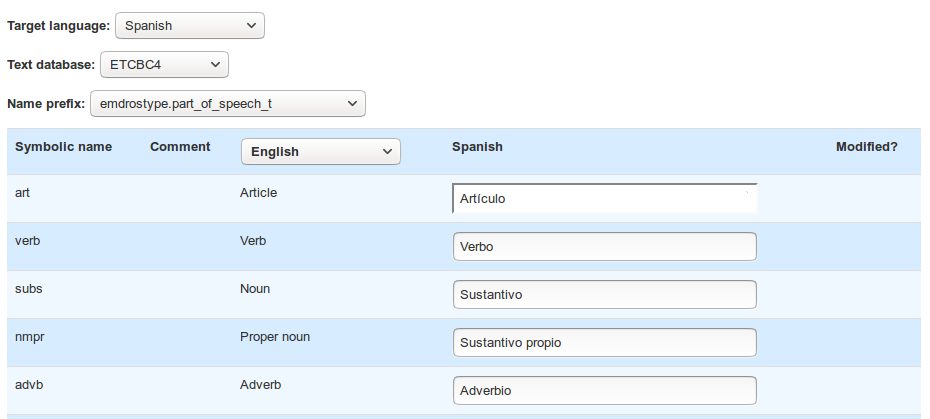
\includegraphics[width=0.9\linewidth]{grammar.png}
\end{center}

From the drop-down menu labelled ``Target language'' select the language you are translating into.
From the drop-down menu labelled ``Text database'' select the database whose grammatical terms you
want to translate. You must provide translations for all databases. Note that the terms for the
ETCBC4 and ETCBC4-translit databases are very similar, but not completely identical.

For convenience, related texts are grouped under a so-called ``name prefix.'' You must provide a
translation for all text under all name prefixes. From the drop-down menu ``Name prefix,'' select
the name prefix you want to work with.

The area below the name prefix selector is divided into five columns:


\begin{flexlabelled}{labeli}{3cm}{*}{0cm}{4cm}{*}
\item[Symbolic name:\hfill] This is used internally by the system.
\item[Comment:] This column may provide some context for translation.
\item[English (or some other language):] This is a drop down menu where you can select an existing
  language to use as the basis for your translation. It is highly recommended that you use English
  for this purpose; otherwise you will be working with something that is already a translation
  from English, and the result may not be the best.
\item[\emph{Target language:}\hfill]  Here you provide your translation.
\item[Modified?] If you have modified an entry, a ``Revert'' button will appear in the ``Modified?''
  column. If you click this button before you save your changes to the server, you will undo any
  changes you have made to that entry.
\end{flexlabelled}

At the bottom of the screen, you will find two buttons, one labelled ``Submit changes'' and one
labelled ``Revert all.'' Clicking ``Submit changes'' will send your updated translations to the server;
clicking ``Revert all'' will undo all the changes you have made but not yet submitted.


\section{Sorting Information}

In the above example the values with the name prefix \emph{emdrostype.part\_of\_speech\_t} have
English translations such as ``Article,'' ``Verb,'' ``Noun,'' and several others. When these values
are displayed by the system, they are normally sorted alphabetically:

\begin{center}
  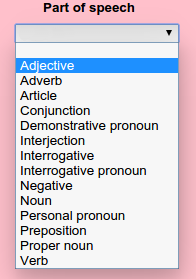
\includegraphics[width=0.3\textwidth]{psp.png}
\end{center}

But sometimes you want another sorting order. If the translation starts with ``\#1,'' ``\#2,'' etc.
these numbers indicate the sort order. You can, for example, specify this (under name prefix
\emph{emdrostype.gender\_t}):

\begin{center}
  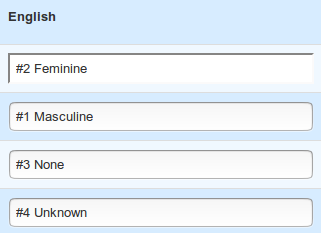
\includegraphics[width=0.3\textwidth]{gendertranslate.png}
\end{center}

Here, the strings ``\#1,'' ``\#2,'' etc. indicate the sorting order. Thus:

\begin{center}
  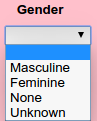
\includegraphics[width=0.148\textwidth]{gender.png}
\end{center}

Be aware that the preferred sorting order in English may not be the preferred sorting order in your language.

\section{Overview of the Name Prefixes}


The following table gives an overview of the name prefixes and their use.

\begin{tabularx}{\textwidth}{@{}>{\footnotesize\ttfamily} l X @{}}
  \toprule
  \headii{\normalsize\textrm{Name prefix}}{Use}\\
  \midrule
  
  info & Database name and copyright information. \\
  emdrosobject\ldots & Grammatical units (such as word, phrase, clause) and their attributes.\\
  emdrostype\ldots & Possible values of the grammatical attributes (for example, the gender
  attribute can be masculine or feminine). \\
  grammargroup\ldots & Groupings of attributes. \\
  grammarfeature\ldots{}, grammarmetafeature\ldots & Names of some grammatical
  attributes. \\
  grammarsubfeature\ldots & Abbreviations of the values of some grammatical attributes. \\
  universe.book& Names of the books of the Bible. \\
  universe.chapter, universe.verse & How to identify a chapter and a verse. \\
  universe.reference & How to format a Bible reference, plus a list of abbreviations of the books of
  the Bible.\\
  
  \bottomrule
\end{tabularx}


%%%%%%%%%%%%%%%%%%%%%%%%%%%%%%%%%%%%%%%%%%%%%%%%%%%%%%%%%%%%%%%
%%%%%%%%%%%%%%%%%%%% Translating a Lexicon %%%%%%%%%%%%%%%%%%%%
\chapter{Translating a Lexicon}

Bible OL uses three lexicons to provide translation of the Hebrew, Aramaic, and Greek words of the
Bible.

To provide a translation, you must log in using an account that has ``translator'' privileges. Then,
from the ``Administration'' menu select ``Translate lexicon.''

You will then see a web page that looks something like this:

\begin{center}
  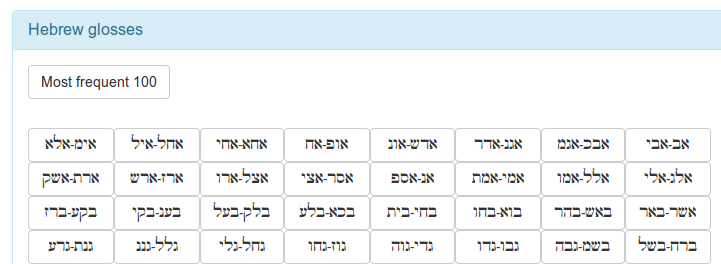
\includegraphics[width=0.9\linewidth]{lexicon.png}
\end{center}

If you scroll down the web page you will find Aramaic and Greek glosses as well.

Clicking the ``Most frequent 100'' button will allow you to provide a translation of the most
frequent 100 words of the language. Alternatively, you can click on one of the many buttons labelled
with letters to bring up a small part of an alphabetically sorted lexicon.

Once you click on a button, you will be shown a web page with a number of words to translate. You
can scroll up the web page to find the list of section selectors again.

For the Hebrew and Aramaic lexicons, the web page will look like this:

\begin{center}
  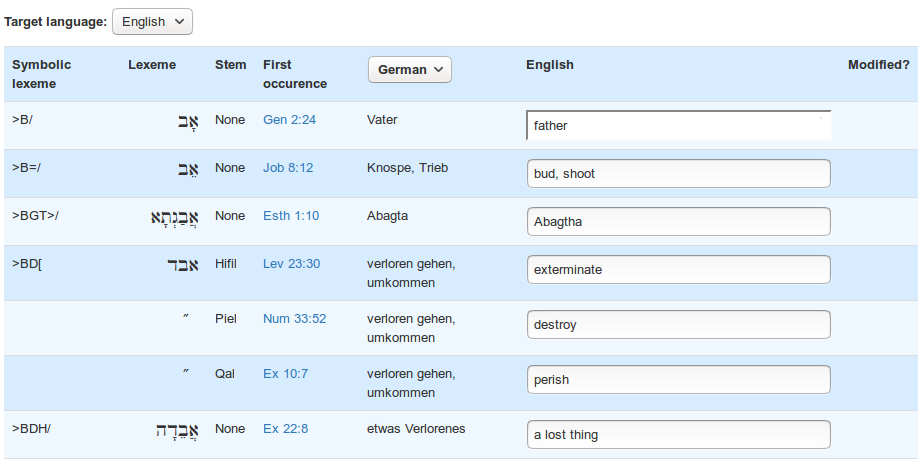
\includegraphics[width=0.9\linewidth]{lexiconHeb.png}
\end{center}

For the Greek lexicon, the web page will look like this:

\begin{center}
  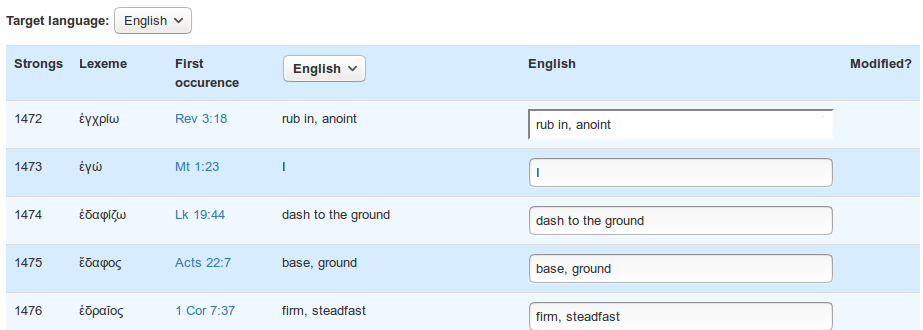
\includegraphics[width=0.9\linewidth]{lexiconGr.png}
\end{center}

From the drop-down menu labelled ``Target language'' select the language you are translating into.

The area below the target language selector is divided into six or seven columns.

For Hebrew and Aramaic the columns are:

\begin{flexlabelled}{labeli}{3cm}{*}{0cm}{4cm}{*}
\item[Symbolic lexeme:\hfill] This is used internally by the system.
\item[Lexeme:] This is Hebrew/Aramaic word to translate.
\item[Stem:] For verbs, the lexicon requires that you provide a translation for each verbal stem.
  Only the stems that actually occur in Bible are listed.
\item[First occurrence:\hfill] A link to the first occurrence of that word in the Bible. (This may
  help you get some context for the word.)
\item[English (or some other language):] This is a drop down menu where you can select an existing
  language to guide you in your translation.
\item[\emph{Target language:}\hfill]  Here you provide your translation.
\item[Modified?] If you have modified an entry, a ``Revert'' button will appear in the ``Modified?''
  column. If you click this button before you save your changes to the server, you will undo any
  changes you have made to that entry.
\end{flexlabelled}

For Greek the columns are:


\begin{flexlabelled}{labeli}{3cm}{*}{0cm}{4cm}{*}
\item[Strongs:] This is the Strong's number for the word
\item[Lexeme:] This is the Greek word to translate.
\item[First occurrence:\hfill] A link to the first occurrence of that word in the Bible. (This may
  help you get some context for the word.)
\item[English (or some other language):] This is a drop down menu where you can select an existing
  language to guide you in your translation. (For Greek we currently only have an English translation,
  therefore the illustration above shows two columns labelled ``English.'')
\item[\emph{Target language:}\hfill]  Here you provide your translation.
\item[Modified?] If you have modified an entry, a ``Revert'' button will appear in the ``Modified?''
  column. If you click this button before you save your changes to the server, you will undo any
  changes you have made to that entry.
\end{flexlabelled}

At the bottom of the screen, you will find two buttons, one labelled ``Submit changes'' and one
labelled ``Revert all.'' Clicking ``Submit changes'' will send your updated translations to the server;
clicking ``Revert all'' will undo all the changes you have made but not yet submitted.




\end{document}

% Local Variables:
% mode: latex
% ispell-dictionary: "british-ize"
% ispell-extra-args: ("--home-dir=/home/claus/Projects/BibleOL/techdoc")
% eval: (auto-fill-mode 1)
% End:
